\documentclass{article}
\usepackage[utf8]{inputenc}
\usepackage{geometry}
\geometry{a4paper, top=3cm, bottom=3cm, left=3cm, right=3cm}
\title{Algorithmic Game Theory}
\author{Giada Gabriele}
\date{July 29, 2022}
\usepackage{amsmath}
\usepackage{amssymb}
\usepackage{graphicx}
\begin{document}

\maketitle
\section{Assignment}
\Large{
The system must select the user who will perform the tour, must define the places that the tour will visit and must define the payments charged to the users. The only constraint we have is the maximum payout. Costs proportional to kilometers should be equally distributed and fixed costs should be based on declared utilities, so we must implement mechanisms that lead to truthful declarations of utilities.
}
\section{Hypothetical mechanism choice}
\Large{
In this section we will show how we arrived at the choice of the mechanism. Studying game theory and related theorems this is the theoretical process that led to the final choice.\\
We start from the definition of \textbf{what} is a Mechanism:
\begin{quote}
    A \textit{Mechanism} (for a Bayesian game setting\\ ($N,O,\Theta,p,u)$) is a pair (A,M), where
    \begin{itemize}
        \item A = $A_1 \times \dots A_n$, where $A_i$ is the set of actions available to agent $i \in N$; and
        \item M : $A \mapsto \Pi(O)$ maps each action profile to a distribution outcomes.
    \end{itemize}
\end{quote}
We want to pay attention on the truthfulness of the game and we know that a \textit{direct mechanism} is one in which the only action to each agent is to announce his private information. Since in a Bayesian game an agent's private information is his type, direct mechanism have $A_i = \Theta_i$, so a direct mechanism is said to be truthful (or incentive compatible) if, for any type vector $\theta$, in equilibrium of the game defined by the mechanism every agent \textit{i}'s strategy is to announce his true type, so that $\hat{\theta}_i = \theta_i$. We can restrict our attention to truthful mechanism,\newpage in this case the \textit{Quasilinear preferences}:
\begin{quote}
    Agents have quasilinear preferences in a \textit{n}-player Bayesian game when the set of outcomes is
    \begin{center}
        $O = X \times \mathbb{R}^n$
    \end{center}
    for a finite set X, and the utility of an agent \textit{i} given joint type $\theta$ is given by
    \begin{center}
        $u_i$(o,$\theta$) = $u_i$(x,$\theta$) - $f_i$($p_i$),
    \end{center}
    where $o = (x,p)$ is an element of $O,\\ u_i : X \times \Theta \mapsto \mathbb{R}$ is an arbitrary function  and $f_i : \mathbb{R} \mapsto \mathbb{R}$ is a strictly monotonically increasing function.
\end{quote}
Then we split the mechanism into two pieces that are linearly related:
\begin{center}
    $u_i(o,\theta) = u_i(x,\theta) - f_i(p_i)$
    \begin{itemize}
        \item $x \in X$ is a discrete non-monetary outcome
        \item $p_i \in R$ is a monetary payment that agent \textit{i} must make to the mechanism
    \end{itemize}
\end{center}
In this way agents care only about the choice selected and about their own payments, not about the monetary payments made by other agents. At this point we can define a \textbf{Quasilinear mechanism}:
\begin{quote}
    A mechanism in the quasilinear setting (for a Bayesian game setting($N,O = X \times \mathbb{R}^n,\Theta,p,u$)) is a triple ($A,\chi,\wp$), where
    \begin{itemize}
        \item $A = A_1 \times \dots A_n$, where $A_i$ is the set of actions available to agent $i \in N$
        \item $\chi : A \mapsto \Pi(X)$ maps each action profile to a distribution over choices, and
        \item $\wp : A \mapsto \mathbb{R}^n$ maps each action profile to a payment for each agent.
    \end{itemize}
\end{quote}
We have split the function M in two functions, $\chi$ is a \textbf{choice rule} and $\wp$ is a \textbf{payment rule}. Now we exploit the \textbf{direct quasilinear mechanism} which is the only setting where each agent is asked to state his type.
\begin{quote}
    A direct quasilinear mechanism (for a Bayesian game setting\\($N,O = X \times \mathbb{R}^n,\Theta,p,u$)) is a pair ($\chi,\wp$); it defines a standard mechanism in the quasilinear setting, where each \textit{i}, $A_i = \Theta_i$.
\end{quote}
At this point we make again assumption that agents' utilities depend only on their own types exploiting the property of \textbf{conditional utility independence}:
\begin{quote}
    A Bayesian game exhibits conditional utility independence if for all agent $i \in N$, for all outcomes $o \in O$ and all pairs of joint types $\theta$ and $\theta' \in \Theta$ for which $\theta_i = \theta'_i$ it holds that \\ $u_i(o,\theta) = u_i(o,\theta')$. 
\end{quote}
And again we go back at the definition of \textbf{truthfulness}, in this case for a quasilinear mechanism:
\begin{quote}
    A quasilinear mechanism is truthful if it is direct and $\forall _i \forall v_i$, agent \textit{i}'s equilibrium strategy is to adopt the strategy $\hat{v}_i = v_i$.
\end{quote}
Established what is truthful for game theory, we can analyze the part relating to costs, \textit{cost sharing}, in particular the most coherent choice for this type of problem is to look at  \textbf{coalitional games} and \textbf{Shapley value}; let's go in order.\\\\
What is a coalitional game:
\begin{quote}
    In coalitional game theory our focus is on what groups of agents, rather than individual agents, can achieve. Given a set of agents, a coalitional game defines how well each group (or coalition) of agents can do for itself. We are not concerned with how the agents make individual choices \\within a coalition, how they coordinate, or any other such detail; we simply take the payoff (or costs, this definition is valuable also for costs - that is our case) to a coalition as given.
\end{quote}
Now we can define some aspects related to the division of costs, starting from the definition of \textbf{feasible payoff}:
\begin{quote}
    Given a coalitional game (N,v), the feasible payoff set is defined as 
    \begin{center}
        \{$x \in \mathbb{R}^N \vert \sum_{i\in N} x_i \le v(N)$\}
    \end{center}
\end{quote}
this set contains all payoff vectors that do not distribute more than the worth of the grand coalition. We can view this as requiring the payoffs to be \textbf{weakly budget balanced}. This balance aspect responds to the goal we set ourselves at the beginning.
\\Therefore for this kind of issue we need to think about group of people who wants to maximize utilities and obtain as outcome the most convenient tour, in a \textit{fair} way. Now we can exploit the definition of \textbf{Shapley Value}:
\begin{quote}
    Given a coalitional game (N,v), the Shapley \\Value of player \textit{i} is given by:
    \begin{center}
    \normalsize{
        $\phi_i(N,v) = \frac{1}{\vert N \vert !} \displaystyle \sum_{S \subseteq \vert N \vert \backslash \{i\}} \vert S \vert!(\vert N \vert -  \vert S \vert - 1)! [v(S \cup \{i\}) - v(S)]$.
    }
    \end{center}
    This expression can be viewed as capturing \\the “average marginal contribution” of agent i, where we average over all the different sequences according to which the grand coalition could be built up from the empty coalition.
\end{quote}
}
\section{Application theory}
\Large{
We must establish some variables of the problem, for example \textbf{how} to evaluate user preferences. Each user has a list of cities, with fixed costs necessary to visit them (the same for all) on which to express their preferences, \textbf{in what way?} Of course from a mathematical point of view this won't be exactly right, we could be more precise with a larger scale but for this example and to not complicate too much the explanation I prefer to stay on a classical ratings-style evaluation, choose a number from 1 to 5. \textbf{What's our best outcome?} First of all, a city can be visited by a particular user if that user can afford to visit that city or that tour of cities, it cannot happen that a user declares a preference and then does not have the possibility to do so, we will demonstrate in the next paragraph how to calculate it. Each rating is equivalent to the utilities of a given city, so the tour that has the highest utility (the one that the majority prefers) wins. For the same utility (if this happens) the one with the lowest cost wins, as often happens in real life, the one on which you save the most wins. At the same cost, the tour that has more cities on the list wins, I would prefer to visit as many cities as possible, as well as have as many people as possible in the vehicle. \\\\At this point we have to clarify some variables in order to be able to respond to the problem requests in the application example part.\\\\
The assignment says that we have to create a game in which a group of people, using a vehicle with \textbf{k} seats, do a tour in some cities. We have the cities but we didn't shaped the problems based on the k constraint. So, exploiting the Shapley value formula we have to change the N variable, in our case it will be:
\begin{center}
    $\displaystyle\sum_{p=1}^k \binom {{\vert N \vert}} {p}$
\end{center}
So in this way we will calculate all the possible games with a group of people $\le$ k, we remain in the coalition game setting and after calculate all the possibilities we will find our best outcome. We have also to define our \textbf{characteristic function}, \textit{v}: it's \textbf{the cost} of the winning tour. What does Shapley value allow us to do indeed? We will have as a result the cost of every game and understand if that is a \textbf{valid} game, people can afford it, or not. In this way we have also a \textbf{fair} game. We don't want any participant to be unhappy, so even if the sum of declared utilities is enough to go on a certain tour is \textit{unfair} if anyone pay, for example, 200 and an other one pay 10 just because the value of the tour is 210, everyone must pay in an "equal" way. Exploiting the Shapley value we start from the bottom, from an empty group, then we calculate the cost of singleton, then couple, etc, in this way passing through singleton we know that everyone in the game can afford it. As the cost of singleton we can pick the cost of the tour with the maximum utility. The Shapley value defined a fair way of dividing the grand coalition’s payment among its members. Also it is not convienent to lie on preferences because if you can afford to go to both Milan and Rome and give 5 to Milan and 4 to Rome and you really want to go to Rome, if Milan wins with maximum utility you go to Milan, it makes no sense, given the statements made, don't tell the truth. However, this analysis ignored questions of stability so we have to define what is the \textbf{core}:
\begin{quote}
    A payoff vector x is in the core of a coalitional game (N,v) if and only if
    \begin{center}
        $\forall S \subseteq N, \displaystyle \sum_{i \in S} x_i \ge v(S)$
    \end{center}
    Thus, a payoff is in the core if and only if no sub-coalition has an incentive to break away from the grand coalition and share the payoff it is able to obtain independently.\\
\end{quote}
At this point we have to clarify some issues.\\\\
We know that Shapley value can be used only in a \textbf{convex} game but we didn't defined the game as convex. There are two theorems about this concept:
\begin{quote}
    (1) Every convex game has a nonempty core.\\\\
    We know that the core may be empty, but if it is not, is the Shapley value guaranteed to lie in the core? The answer in general is no, but the following theorem gives us a sufficient condition for this property to hold. We already know from this theorem that the core of convex games is nonempty. The following theorem further tells us that for such games the Shapley value belongs to that set.\\\\
    (2) In every convex game, the Shapley value is in the core.
\end{quote}
So we are not able to define and be sure that this game is convex, we assume that and we declare that the Shapley value is in the core based on these theorems.\\\\
Summarizing, to solve our problem we need the following variables:
\begin{itemize}
    \item preferences (utility) : 1 to 5
    \item v : cost of each city - fixed and given as input
    \item N : maximum number of possible games
    \item  $\displaystyle\sum_{p=1}^k \binom {{\vert N \vert}} {p}$ : possible games in a maximum of k vehicle seats
\end{itemize}
}
\section{Application workflow}
\begin{figure}[htbp!]
\centering
  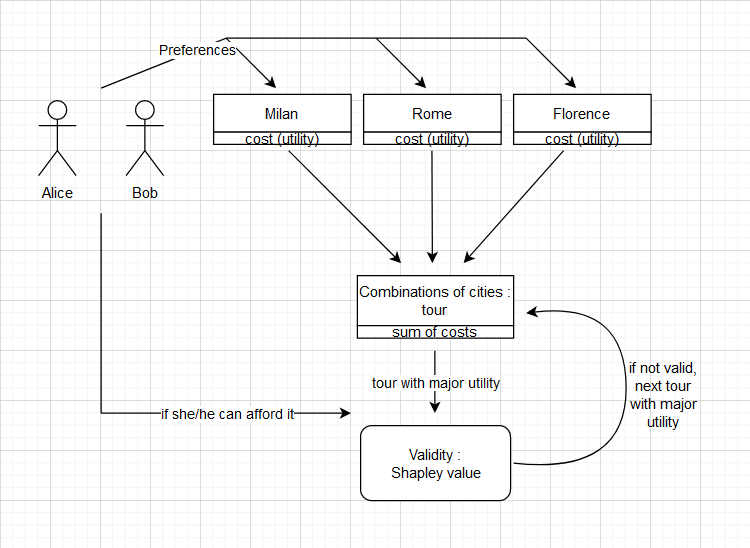
\includegraphics[width=\linewidth]{workflow.png}
  \label{fig:workflow}
\end{figure}
\section{Application example}
\Large{
Let's suppose we have 2 people - Alice and Bob, and 3 cities - Milan(M), Rome(R) and Florence(F). Alice and Bob will declare a utility related to each city, like:
\begin{center}
\begin{tabular}{ |c|c|c|c| } 
 \hline
  & M & R & F \\ 
 \hline
 Alice & 5 & 4 & 3\\ 
 \hline
 Bob & 5 & 4 & 2\\ 
 \hline
\end{tabular}\newpage
\end{center}
Alice has 250 as maximum payment, Bob has 350. The costs related to cities are:
\begin{center}
\begin{tabular}{ |c|c| } 
 \hline
 M & 400 \\ 
 \hline
 R & 300\\ 
 \hline
 F & 200\\ 
 \hline
 MR & 500\\ 
 \hline
 MF & 450\\ 
 \hline
 RF & 370\\ 
 \hline
 MRF & 700\\ 
 \hline
\end{tabular}
\end{center}
Now we have to calculate \textit{v}. \\The empty group has v = 0, then \\v(\{A\}) = 200, \\we look at utilities and we know where she prefers to go, then we look at the "wallet" and we know if she can afford it, in this case Florence it's the "least desirable" but is the only one; same reasoning for Bob.\\
v(\{B\}) = 300 (he can afford to go to Rome, and he prefers Rome to Florence)\\
v(\{A\} $\cup$ \{B\}) = \textbf{?} \\\\
We calculate the value of the group using \textit{Shapley value}.\\
First, the most valid (with highest utility) tour is MR, because MRF = 700 $\ge$ 250+350, now we have to verify if there will be a fair division of costs.\\
Considering $\displaystyle\sum_{p=1}^k \binom {\vert N \vert} {p}$, every single valid coalition will be represented by a variable \textbf{G} so in this case we have:
\begin{center}
   \normalsize{
        $\phi_i(G,v) = \frac{1}{G!} \displaystyle \sum_{S \subseteq G \backslash \{i\}} \vert S \vert!(G -  \vert S \vert - 1)! [v(S \cup \{i\}) - v(S)]$.
    }
\end{center}
S(\{A\}) = $\frac {500 - 300} {2}$ + $\frac {200 - 0} {2}$  = 200
\begin{quote}
    we know that the other S should be 300 because budget balance, let's check:
\end{quote}
S(\{B\}) = $\frac {500 - 200} {2}$ + $\frac {300 - 0} {2}$ = 300
}
\\\\Both are valid because S(\{A\}) = 200 $<$ 250 (Alice's "wallet") and \\S(\{B\}) = 300 $<$ 350 (Bob's "wallet"). \\\\If these conditions were not met we had to calculate the next tour with the major utility. Of course from a computer science point of view this is not an ideal condition, being recursive, having to calculate everything every time and being able to fall into a very large case is expensive (computationally speaking) but it is still a concrete solution to solve this type of problem.
\end{document}